% {{0, 1, 1},
% {1, 18, 18},
% {2, 243, 243},
% {3, 3240, 3240},
% {4, 43254, 43239},
% {5, 577368, 574908},
% {6, 7706988, 7618438},
% {7, 102876480, 100803036},
% {8, 1373243544, 1332343288},
% {9, 18330699168, 17596479795},
% {10, 244686773808, 232248063316},
% {11, 3266193870720, 3063288809012},
% {12, 43598688377184, 40374425656248},
% {13, 581975750199168, 531653418284628},
% {14, 7768485393179328, 6989320578825358},
% {15, 103697388221736960, 91365146187124313},
% {16, 1384201395738071424, 1100000000000000000},
% {17, 18476969736848122368, 12000000000000000000},
% {18, 246639261965462754048, 29000000000000000000},
% {19, 3292256598848819251200, 1500000000000000000},
% {20, 43946585901564160587264, 300000000}}

% квинтиллионом


For balanced dataset, we do $K \in [1, \sub{D}{est}]$ random steps from $V_0$.
\vfill

\begin{minipage}{0.55\textwidth}
It is important to carefully choose $\sub{K}{max} \sim \sub{D}{est}$.
    \begin{figure}[h]
        \centering
        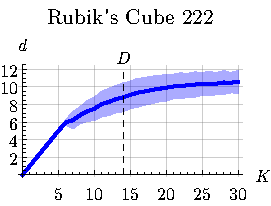
\includegraphics{imgs/dK_dist.pdf}
        %\caption{}
        %\label{fig:}
    \end{figure}
    
\end{minipage}
\hfill
\begin{minipage}{0.4\textwidth}
	\begin{figure}[h]
	    \centering
	    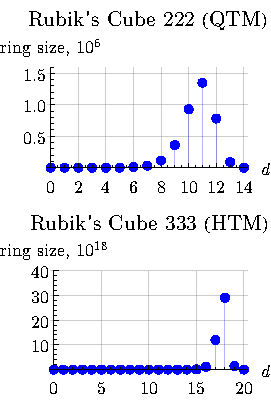
\includegraphics{imgs/d_dist.pdf}
	    %\caption{}
	    %\label{fig:}
	\end{figure}
\end{minipage}


